\documentclass[tikz,border=4pt]{standalone}
\usepackage[T1]{fontenc}
\usepackage{lmodern}
\renewcommand{\familydefault}{\sfdefault}
\usetikzlibrary{shapes.geometric,positioning,arrows.meta,calc}
\tikzset{
  node distance=6mm,
  every node/.style={font=\footnotesize,align=center,execute at begin node={\hyphenpenalty=10000\relax}},
  base/.style={draw=gray!60,fill=gray!12,minimum height=7mm,inner sep=2pt},
  term/.style={base,rounded corners=3.5mm,text width=30mm},
  proc/.style={base,text width=32mm},
  err/.style={base,text width=30mm,fill=gray!22},
  io/.style={base,trapezium,trapezium left angle=72,trapezium right angle=108,trapezium stretches=true,text width=28mm},
  dec/.style={base,diamond,aspect=2.4,text width=27mm,inner sep=0pt},
  go/.style={-{Stealth[length=2mm]},draw=gray!55!black},
  lab/.style={font=\scriptsize,fill=white,inner sep=1pt},
}

\begin{document}
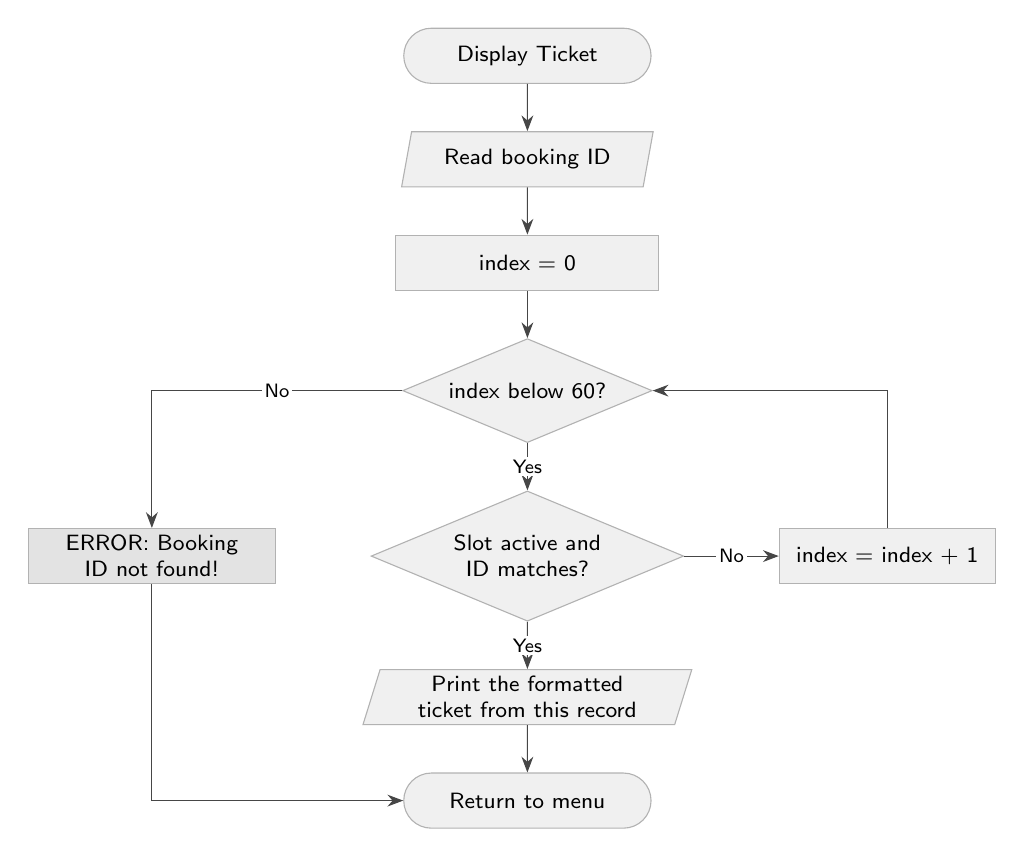
\begin{tikzpicture}
\node[term] (s) {Display Ticket};
\node[io,below=of s] (r) {Read booking ID};
\node[proc,below=of r] (i) {index = 0};
\node[dec,below=of i] (d) {index below 60?};
\node[dec,below=of d] (m) {Slot active and ID matches?};
\node[proc,right=12mm of m,text width=26mm] (n) {index = index + 1};
\node[err,left=12mm of m] (e) {ERROR: Booking ID not found!};
\node[io,below=of m,text width=36mm] (t) {Print the formatted ticket from this record};
\node[term,below=of t] (x) {Return to menu};
\draw[go] (s)--(r);\draw[go] (r)--(i);\draw[go] (i)--(d);
\draw[go] (d)--node[lab]{Yes}(m);
\draw[go] (d.west)-|node[lab,pos=.25]{No}(e.north);
\draw[go] (m)--node[lab]{No}(n);
\draw[go] (n.north)|-(d.east);
\draw[go] (m)--node[lab]{Yes}(t);
\draw[go] (t)--(x);
\draw[go] (e.south)|-(x.west);
\end{tikzpicture}
\end{document}
